\documentclass[11pt]{article}
\usepackage[T1]{fontenc}
\usepackage{lmodern,amsmath,amssymb,amsthm,mathtools,booktabs,array,graphicx}
\usepackage[margin=1in]{geometry}
\usepackage{microtype,xcolor,enumitem,xurl}
\usepackage[pdfencoding=auto,psdextra,hidelinks]{hyperref}
\usepackage{fancyhdr}
\definecolor{ink}{HTML}{164F61}
\definecolor{accent}{HTML}{AD633B}
\pagestyle{fancy}\fancyhf{}
\fancyhead[L]{\small Positive averaging at Dirichlet zeros}
\fancyhead[R]{\small Research report}
\fancyfoot[C]{\thepage}
\setlength{\headheight}{14pt}
\setlength{\emergencystretch}{2em}
\allowdisplaybreaks[2]
\setlist{nosep}
\newtheorem{theorem}{Theorem}[section]
\newtheorem{lemma}[theorem]{Lemma}
\newtheorem{corollary}[theorem]{Corollary}
\newtheorem{proposition}[theorem]{Proposition}
\theoremstyle{remark}\newtheorem{remark}[theorem]{Remark}
\newcommand{\R}{\mathbb R}\newcommand{\C}{\mathbb C}
\newcommand{\dd}{\,\mathrm d}
\hypersetup{pdftitle={Positive averaging with logarithmic support at Dirichlet zeros},
 pdfauthor={Research report prepared for Vladimir Reshetnikov}}
\title{\textcolor{ink}{Positive averaging with logarithmic support\\at Dirichlet zeros}\\[5pt]
\large Optimal support order, stable finite constructions,\\and simultaneous prime-error averaging on a polylogarithmic range}
\author{Research report prepared for Vladimir Reshetnikov}
\date{26 November 2026}
\begin{document}
\maketitle
\begin{abstract}
For any fixed finite family of Dirichlet $L$-functions, we construct a
positive, even, compactly supported probability density whose Fourier
transform vanishes at every prescribed nonzero zero ordinate up to height
$B$, including prescribed multiplicities. Its support has half-width
$O(\log B)$, and its Fourier transform is at most
$\exp(-cB\log B)$ at every real frequency of magnitude at least $B$.
This replaces the $O((\log B)^2)$ support budget in the inspected ProveIt
balancing report. Jensen's formula proves the logarithmic order optimal;
even cancellation without multiplicity at the distinct zeta ordinates
requires half-width at least $(5/12-o(1))\log B$ under RH.
The finite construction colors the frequencies into separated sets and
solves uniformly well-conditioned Fourier interpolation systems while
retaining a quantitative positive-density margin. Using the proved
Dirichlet GRH and a sharpened ramp explicit formula, the construction
simultaneously averages all reduced-residue prime errors using scales
between $X/(\log X)^C$ and $X(\log X)^C$, with weighted error
$O(X^{-1}(\log X)^A)$ after retaining the central-zero bias.
The proofs are complete human-readable arguments; the new result is not
Lean-formalized. Classical interpolation and zero-counting inputs are
credited. Novelty is established relative to the inspected research
packets; worldwide priority of the precise arithmetic formulation is
not certified.
\end{abstract}

\section{The result and its relation to the requested sources}

The central advance is a quantitative positive averaging theorem. A finite
list of many oscillations can be cancelled using nonnegative averaging
weights whose support is controlled by the list's \emph{local density},
instead of by the sum of the reciprocals of all its frequencies. For
Dirichlet zero ordinates, local density is logarithmic in the height.
This yields an order-sharp improvement over the supplied construction.

\subsection{Precise contribution}

Let $\mathcal F$ be a fixed finite family of primitive Dirichlet characters,
closed under conjugation. Write $\Lambda_B$ for the signed nonzero
imaginary parts of their nontrivial zeros up to height $B$, with aggregate
multiplicity. Our construction supplies even probability densities
$\mu_B$ such that
\begin{equation}\label{eq:intro-main}
\begin{gathered}
 \operatorname{supp}\mu_B\subset[-C_{\mathcal F}\log B,C_{\mathcal F}\log B],
 \qquad \operatorname{ord}_{\gamma}\widehat\mu_B\ge m_{\Lambda_B}(\gamma),\\
 \sup_{|\omega|\ge B}|\widehat\mu_B(\omega)|
       \le e^{-c_0B\log B},\qquad c_0=-\log(\sin1)>0,
\end{gathered}
\end{equation}
for $B$ sufficiently large. The support constant depends on the fixed
family. Its optimum value is not determined here.
The filter statement concerns ordinates and needs no RH. GRH supplies
their use as real Fourier frequencies in the prime-error application.

Under RH, any positive probability measure cancelling the same distinct zeta
ordinates, even without matching their multiplicities, has half-width
\[
 H_B\ge(5/12-o(1))\log B.
\]
If the cancellation order must match zero multiplicity, the stronger bound is
\[
 H_B\ge\tfrac12\log B-\tfrac12\log(2\pi)-1
             -O(\log^2 B/B).
\]
The first bound uses the proved part of Montgomery's pair-correlation
work, not the pair-correlation conjecture. The second uses only the
classical zero count and Jensen's formula.

\begin{center}
\small
\begin{tabular}{@{}p{.27\textwidth}p{.31\textwidth}p{.34\textwidth}@{}}
\toprule
Quantity & Inspected balancing packet & This report\\
\midrule
Logarithmic support at cutoff $B$ & $O_q((\log B)^2)$ & $O_q(\log B)$, optimal order\\[3pt]
Low zero modes & Exactly cancelled & Exactly cancelled, with optional multiplicity\\[3pt]
High-frequency multiplier & $\exp(-cB\log B)$ & $\exp(-c_0B\log B)$\\[3pt]
Scales for prime sums near $X$ & $X\exp(\pm O_q((\log\log X)^2))$ & $X(\log X)^{\pm O_q(1)}$\\[3pt]
Weighted ramp remainder & $O_{q,\varepsilon}(X^{-1+\varepsilon})$ & $O_q(X^{-1}(\log X)^A)$\\
\bottomrule
\end{tabular}
\end{center}
The comparison is with the center-independent kernel in
\cite{priorbalance}. That report also proves a different, center-dependent
exact convex balancing theorem in bounded windows; that result is not
superseded or contradicted here. The constants of the present construction
are conservative, so its support need not be smaller at small cutoffs.

\subsection{What the Lean repository proves and what we use}

The requested repository \cite{grh} was inspected at commit
\path{72fead102f663d5c7a407964a13dc0cf9d977207}.
Its exported statements include Mathlib's \texttt{RiemannHypothesis},
nonvanishing of Dirichlet $L$-functions to the right of $1/2$ except at
the principal pole, and critical-strip zero location for all Dirichlet
characters, including imprimitive ones. Its toolchain is Lean
\texttt{v4.35.0}, with Mathlib pinned at
\path{56a005855ea17e0b0958f73ec801ae140b0a1679}.
The joint Lean FRO and Mathlib Initiative statement endorses the original
proof and statement \cite{leanstatement}; independent verification records
for the exact shorter editions are supplied by Sutherland \cite{sutherland}.
The selected source files and their Git blob identifiers were checked
against the pinned snapshot. No local rebuild of the entire development
was performed for this report.

The source route is mathematically relevant. Upper and lower bounds for
the same corrected logarithmic covolume cancel their common main term.
The resulting one-sided bound controls a remainder built from nonnegative
ramp-weighted prime sums. A Mellin transform identifies its poles with differences of
zero multiplicities. An auxiliary quadratic twist removes cancellation
in the finite region being examined, and Landau positivity excludes the
remaining poles. These steps can be inspected in
\path{New/Reduction/MainInequality.lean},
\path{New/Reduction/OneSidedBound.lean},
\path{New/Reduction/Zeros/PrimeError.lean}, and
\path{New/Reduction/Zeros/Criterion.lean} under \path{grh/src/}.

We use the proved Dirichlet GRH and the analytic ideas of positive
smoothing, ramp weights, and zero-multiplicity bookkeeping. The new
argument does not require an extension of the arithmetic-geometric
covolume machinery. Nor does it assert GRH for arbitrary nonabelian
Artin or automorphic $L$-functions. The requested Wikipedia page
\cite{wiki} was used for orientation; the proof scope and verification
claims were traced to primary sources.

\subsection{How repetition was avoided}

The ProveIt directory was inspected at commit
\path{dedc2966ea6f59cc0a8fd0327d68cda31bce6df1}.
Its catalogue contains two batches, of 61 and 42 research packets, and
explicitly says their placement did not constitute mathematical or Lean
verification \cite{catalogue}. Nine closely relevant reports were read
in full; the accompanying inventory records their blob identifiers.
They already include arbitrary-shift covariance, spectral coercivity,
polynomial zero-divisor rigidity, prime-peak recurrence, and a sharp
scalar coalescence law. Those results are not presented here as new.
The specific quantitative advance is the support and accuracy theorem
above, with a complete positivity-preserving construction and matching
support order.

% Input fragment: requires amsmath, amssymb, amsthm and theorem/lemma/corollary environments.
% All statements and proofs below were independently derived for this packet.

\section{Positive Fourier annihilation with logarithmic support}
\label{sec:annihilation}

Our Fourier convention for a finite measure on the real line is
\[
 \widehat\mu(z)=\int_{\mathbb R}e^{izt}\,d\mu(t).
\]
If $\mu$ is supported on $[-H,H]$, this is entire. A zero of order
at least $r$ at $\lambda$ means
$\widehat\mu^{(j)}(\lambda)=0$ for $0\le j<r$.
For a finite symmetric multiset $\Lambda\subset\mathbb R\setminus\{0\}$,
write $m_\Lambda(\lambda)$ for its multiplicity. Symmetric means that
$m_\Lambda(-\lambda)=m_\Lambda(\lambda)$.

\subsection{A uniformly positive interpolating density}

\begin{lemma}[Separated frequencies]\label{lem:separated-filter}
Let $\Gamma\subset\mathbb R\setminus\{0\}$ be a finite symmetric set,
and suppose that the distinct points of $\Gamma\cup\{0\}$ are at least
$\delta>0$ apart. Put $A=4\pi/\delta$ and
\[
 g_A(t)=\frac1A\left(1-\frac{|t|}{A}\right)_+,
 \qquad
 f_A(z)=\left(\frac{\sin(Az/2)}{Az/2}\right)^2.
\]
There is an even probability density $w_\Gamma$ on $[-A,A]$ such that
\begin{equation}\label{eq:positive-envelope}
 \frac56 g_A(t)\le w_\Gamma(t)\le\frac65 g_A(t),
 \qquad
 \widehat w_\Gamma(\lambda)=0\quad(\lambda\in\Gamma).
\end{equation}
It is specified by a real linear system with a matrix whose induced
$\ell^1$ distance from the identity is at most $1/12$.
\end{lemma}

\begin{proof}
The density $g_A$ is the convolution of two uniform densities on
$[-A/2,A/2]$, so its Fourier transform is $f_A$. In particular, for
real $x\ne0$,
\[
 0\le f_A(x)\le\frac4{A^2x^2},\qquad f_A(0)=1.
\]
Index the coordinates by the distinct points of $\Gamma$, and define
\[
 M_{\lambda\kappa}=f_A(\lambda-\kappa),
 \qquad b_\lambda=f_A(\lambda).
\]
For each fixed $\kappa$, the $j$th point to its right is at distance
at least $j\delta$, and the same holds on its left. Consequently
\begin{align}
 \|M-I\|_1
 &\le \frac8{A^2\delta^2}\sum_{j\ge1}\frac1{j^2}
 =\frac{4\pi^2}{3A^2\delta^2}=\frac1{12},\label{eq:matrix-bound}\\
 \|b\|_1
 &\le \frac8{A^2\delta^2}\sum_{j\ge1}\frac1{j^2}
 =\frac1{12}.\label{eq:rhs-bound}
\end{align}
The second estimate uses separation from the additional point $0$.
The Neumann series makes $M$ invertible and gives
\[
 a=-M^{-1}b,\qquad
 \|a\|_1\le\frac{1/12}{1-1/12}=\frac1{11}.
\]
The data are real, so $a$ is real. Simultaneous replacement of
$\lambda,\kappa$ by $-\lambda,-\kappa$ preserves $M$ and $b$;
uniqueness gives $a_{-\lambda}=a_\lambda$. Therefore
\[
 Q(t)=1+\sum_{\lambda\in\Gamma}a_\lambda e^{-i\lambda t}
\]
is real and even, and $10/11\le Q(t)\le12/11$ for every $t$.
Its weighted integral
\[
 Z=\int_{\mathbb R}g_A(t)Q(t)\,dt
   =1+\sum_{\lambda\in\Gamma}a_\lambda f_A(\lambda)
\]
also lies between $10/11$ and $12/11$. Set
$w_\Gamma=g_AQ/Z$. It is an even probability density, and comparison
of these two bounds proves \eqref{eq:positive-envelope}. Finally,
\[
 \widehat w_\Gamma(\kappa)
 =\frac1Z\left(f_A(\kappa)+
       \sum_{\lambda\in\Gamma}a_\lambda
                      f_A(\kappa-\lambda)\right)=0
 \qquad(\kappa\in\Gamma),
\]
by $Ma=-b$.
\end{proof}

The constant $4\pi$ is convenient rather than optimized. The proof
uses finite matrices and a quantitative positivity margin; it invokes
no zero-separation conjecture for any $L$-function.

\subsection{Clustering, multiplicities, and uniform attenuation}

\begin{theorem}[A finite positive filter with an explicit support bound]
\label{thm:finite-filter}
Let $B>0$, and let $\Lambda$ be a finite symmetric multiset in
$[-B,B]\setminus\{0\}$. Choose $\delta>0$ such that every positive
element of $\Lambda$ is at least $\delta$. Define the local occupancy
\[
 K=\sup_{x\ge0}\sum_{\substack{\lambda>0\\x<\lambda\le x+\delta}}
                      m_\Lambda(\lambda).
\]
For every integer $N\ge0$, there is an even probability measure
$\mu_{\Lambda,N}$ supported on
\begin{equation}\label{eq:finite-support}
 [-H,H],\qquad H=\frac{4\pi K}{\delta}+\frac NB,
\end{equation}
whose transform satisfies
\begin{align}
 \operatorname{ord}_{z=\lambda}\widehat\mu_{\Lambda,N}(z)
   &\ge m_\Lambda(\lambda)
       &&(\lambda\in\Lambda),\label{eq:jet-zeros}\\
 |\widehat\mu_{\Lambda,N}(\omega)|
   &\le (\sin1)^N
       &&(\omega\in\mathbb R,\ |\omega|\ge B).\label{eq:tail-attenuation}
\end{align}
If $K+N>0$, the measure can be chosen absolutely continuous.
For $\Lambda$ empty, take $K=0$.
\end{theorem}

\begin{proof}
Process the positive occurrences of $\Lambda$ in nondecreasing order,
and color them greedily using $K$ colors. A color may be reused only
when its previous occurrence is at distance at least $\delta$.
At a current occurrence $\lambda$, every unavailable color has an
occurrence in $(\lambda-\delta,\lambda]$ that was processed earlier.
Together with the current occurrence there are at most $K$ such
occurrences. Thus at most $K-1$ colors are unavailable, and the
procedure succeeds. This argument includes repeated ordinates: equal
occurrences must receive different colors. The case
$\lambda-\delta<0$ causes no difficulty because no positive occurrence
is smaller than $\delta$.

For each nonempty color, reflect its positive set through the origin.
This gives a symmetric set $\Gamma_k$ with pairwise distance at least
$\delta$, also separated from $0$. In particular, the distance between
a positive and a negative point is at least $2\delta$. Apply
Lemma~\ref{lem:separated-filter} and convolve the resulting probability
measures. Their convolution $\nu$ is even, positive, and supported on
$[-4\pi K/\delta,4\pi K/\delta]$. Each occurrence of $\lambda$ belongs
to one color whose factor has a zero there. Since the Fourier transform
of a convolution is a product, its order at $\lambda$ is at least
$m_\Lambda(\lambda)$.

Let $u_B$ be the uniform probability measure on $[-1/B,1/B]$, and set
\[
 \mu_{\Lambda,N}=\nu*u_B^{*N},\qquad
 \widehat u_B(\omega)=\frac{\sin(\omega/B)}{\omega/B}.
\]
An empty convolution is the point mass at $0$. Convolution adds the
support radii and preserves the zero orders. On $1\le x\le\pi$,
$\sin x/x$ decreases from $\sin1$ to $0$, since the derivative's
numerator $x\cos x-\sin x$ has derivative $-x\sin x<0$. For
$x\ge\pi$, $|\sin x/x|\le1/\pi<\sin1$. Hence
\[
 \sup_{|x|\ge1}\left|\frac{\sin x}{x}\right|=\sin1<1.
\]
Every probability measure has Fourier transform of modulus at most
$1$ on the real axis. This proves \eqref{eq:tail-attenuation}, and the
absolute-continuity claim follows from the construction.
\end{proof}

There is a useful accuracy form of the same theorem. Set
$c_0=-\log(\sin1)>0$. Given $0<\varepsilon<1$, choose
$N=\lceil c_0^{-1}\log(1/\varepsilon)\rceil$. Then the tail is at most
$\varepsilon$ and
\[
 H\le\frac{4\pi K}{\delta}
       +\frac{\log(1/\varepsilon)}{c_0B}+\frac1B.
\]
Thus the support cost for exact low-frequency interpolation and the
additional cost for high-frequency damping are explicitly separated.

\begin{corollary}[Polynomial modes and frequency error]
\label{cor:jet-robustness}
Let $\mu$ be a compactly supported finite measure. If $\widehat\mu$ has a zero of order at least $r$ at a real
$\lambda$, then for every polynomial $P$ of degree less than $r$ and
every real $T$,
\[
 \int P(T+t)e^{i\lambda(T+t)}\,d\mu(t)=0.
\]
If moreover $\mu$ is a probability measure on $[-H,H]$, then for every
real $\eta$,
\begin{equation}\label{eq:frequency-robustness}
 |\widehat\mu(\lambda+\eta)|
 \le\min\left(1,\frac{(H|\eta|)^r}{r!}\right).
\end{equation}
\end{corollary}

\begin{proof}
Compact support permits differentiation under the integral:
$\widehat\mu^{(j)}(\lambda)=\int(it)^je^{i\lambda t}\,d\mu(t)$.
Expand $P(T+t)$ to obtain the first assertion. For the second, subtract
the first $r$ Taylor terms of $e^{i\eta t}$ inside the integral; their
integrals vanish. Taylor's integral remainder along the real axis is
bounded by $|\eta t|^r/r!$, because every derivative of $e^{ix}$ has
modulus one. Integrate and use $|t|\le H$. The additional bound $1$ is
the probability-measure estimate.
\end{proof}

\subsection{Application to Dirichlet zero ordinates}

Fix a finite family $\mathcal F$ of primitive Dirichlet characters
closed under complex conjugation, with the primitive trivial
character allowed. Let
$\Lambda_B$ be the multiset of all their nonzero zero ordinates
$\gamma=\Im\rho$ with $|\gamma|\le B$, counting multiplicity in each
$L$-function and adding multiplicities when zeros are shared.
Closure under conjugation makes $\Lambda_B$ symmetric. Zeros with
ordinate zero are excluded: no probability measure can have Fourier
transform zero at $0$. Under GRH these are precisely the central zeros.

The standard local zero bound \cite{Davenport} gives
\begin{equation}\label{eq:local-zero-bound}
 \sum_{\chi\in\mathcal F}
 \#\{\rho:L(\rho,\chi)=0,\ 0<\Re\rho<1,\ t<\Im\rho\le t+1\}
 \ll_{\mathcal F}\log(t+3),\qquad t\ge0,
\end{equation}
with multiplicities. Analyticity gives a positive minimum nonzero
absolute ordinate for this fixed finite family. Choose a fixed
$\delta\le1$ no larger than that minimum. Its occupancy $K_B$ in
Theorem~\ref{thm:finite-filter} is $O_{\mathcal F}(\log(B+3))$.
Taking $N=\lceil B\log B\rceil$, for $B\ge2$, proves the following.

\begin{theorem}[Logarithmic support for Dirichlet zero filters]
\label{thm:dirichlet-filter}
For the fixed conjugation-closed family $\mathcal F$, there are even probability densities $\mu_B$, $B\ge2$, with support radius
\[
 H_B=O_{\mathcal F}(\log(B+3)),
\]
which vanish at every prescribed nonzero zero ordinate up to $B$
to at least its aggregate multiplicity, and satisfy
\[
 \sup_{|\omega|\ge B}|\widehat\mu_B(\omega)|
 \le e^{-c_0B\log B},\qquad c_0=-\log(\sin1)>0.
\]
No assumption about simple zeros, distinct zeros of different
$L$-functions, or linear independence of ordinates is required.
\end{theorem}

This theorem about imaginary parts of zeros is unconditional: ordinates
are real numbers by definition. Dirichlet GRH is needed below to identify
the nontrivial-zero contributions to prime errors with pure Fourier modes.
The arithmetic input for the support estimate is the classical local zero
count, which follows from the standard zero-counting formula \cite{Davenport}. If the initial family is not closed
under conjugation, first adjoin its conjugates; the conclusion then
applies simultaneously to the original family.

\subsection{Why the logarithmic order cannot be reduced}

The following lower bound applies even to nonsymmetric probability
measures and even to a measure whose supporting interval is not
centered at the origin: translate the measure to center that interval,
which multiplies its Fourier transform by a nonvanishing exponential.

\begin{lemma}[Jensen support bound]\label{lem:jensen-support}
Let $\mu$ be a probability measure supported on $[-H,H]$. Suppose its
Fourier transform vanishes at every point of a finite symmetric
multiset $\Lambda\subset[-B,B]\setminus\{0\}$ to at least the
specified multiplicity. Then
\begin{equation}\label{eq:jensen-support}
 H\ge\frac{\pi}{2B}
       \sum_{\lambda\in\Lambda}\log\frac{B}{|\lambda|}
  =\frac\pi B\int_0^B\frac{N_\Lambda(t)}t\,dt,
\end{equation}
where $N_\Lambda(t)$ counts positive occurrences up to $t$.
\end{lemma}

\begin{proof}
Put $F(z)=\widehat\mu(z)$. Then $F(0)=1$ and
$|F(Re^{i\theta})|\le e^{HR|\sin\theta|}$. Jensen's formula, first
for radii without boundary zeros, gives
\[
 \sum_{F(z)=0,\ |z|<R}\log\frac R{|z|}
 =\frac1{2\pi}\int_0^{2\pi}\log|F(Re^{i\theta})|\,d\theta
 \le\frac{2HR}\pi.
\]
Keep just the prescribed zeros and let $R$ decrease to $B$ through
admissible radii. Zeros exactly at $B$ contribute zero in the limit.
This proves the first inequality. The equality is the elementary
identity
$\sum_{0<\lambda\le B}m_\Lambda(\lambda)\log(B/\lambda)
 =\int_0^BN_\Lambda(t)\,dt/t$, together with symmetry.
\end{proof}

For the zeta function, let $N(T)$ count positive ordinates with
multiplicity. The Riemann--von Mangoldt formula \cite{Montgomery,CGG} is
\[
 N(T)=\frac{T}{2\pi}\log\frac{T}{2\pi}
       -\frac{T}{2\pi}+O(\log(T+2)).
\]
Substitution into \eqref{eq:jensen-support} gives the explicit
asymptotic obstruction
\begin{equation}\label{eq:zeta-support-lower}
 H\ge\frac12\log B-\frac12\log(2\pi)-1
       +O\!\left(\frac{\log^2 B}{B}\right)
\end{equation}
for multiplicity-preserving cancellation of all zeta ordinates up to
$B$. Here the $O$ term means that the right-hand side can be decreased
by an absolute constant times $\log^2B/B$ to obtain an inequality.
More generally, for $d=|\mathcal F|$ with conductors $f_\chi$,
the corresponding aggregate-multiplicity lower bound is
\begin{equation}\label{eq:family-support-lower}
 H\ge\frac d2\log B+
       \frac12\sum_{\chi\in\mathcal F}\log\frac{f_\chi}{2\pi}
       -d+O_{\mathcal F}\!\left(\frac{\log^2 B}{B}\right).
\end{equation}
Indeed the sum of the positive zero-counting functions has the same
Riemann--von Mangoldt main terms, summed over the family. The
conjugation closure pairs any differences between positive and
negative ordinates. Thus the upper bound of
Theorem~\ref{thm:dirichlet-filter} has the optimal order $\log B$;
no claim is made that its leading constant is optimal.

\paragraph{Ordinary cancellation without prescribed multiplicity.}
For completeness, the logarithmic obstruction persists even when one
asks for only a simple Fourier zero at each distinct zeta ordinate.
Under RH, Montgomery's proved pair-sum formula \cite{Montgomery,CGG} implies
\[
 M_2(T):=\sum_{\substack{0<\gamma\le T\\\gamma\ {\text{distinct}}}}m_\gamma^2
 \le\left(\frac43+o(1)\right)N(T).
\]
This uses only the proved Fourier-support range of his theorem,
not the pair-correlation conjecture: the nonnegative squared-sinc
pair sum with parameter $0<a<1$ has asymptotic
$(a^{-1}+a/3)T\log T/(2\pi)$, and its equal-ordinate terms are exactly
$M_2(T)$; then let $a\uparrow1$ after $T\to\infty$.
For each integer $m\ge1$, $m-1\le(m^2-m)/2$. Hence, writing $D(T)$
for the number of distinct positive ordinates,
\[
 D(T)\ge\frac{3N(T)-M_2(T)}2
       \ge\left(\frac56-o(1)\right)N(T).
\]
Use $D(t)$ in Jensen's formula and integrate to obtain
\begin{equation}\label{eq:distinct-support-lower}
 H\ge\left(\frac5{12}-o(1)\right)\log B.
\end{equation}
Therefore even the weaker task of ordinary zero cancellation has
minimal support radius of order $\log B$. These constants are
convenient rigorous lower bounds, not asserted to be the best
constants available from the zero-density literature.


\section{Uniform averaging of arithmetic signals}\label{sec:applications}

The distinction between a single rule that works at every translate and a rule
chosen separately at each translate is essential.  The kernels constructed
above are independent of the center of the averaging interval.  Their
application therefore gives uniform control of an entire almost periodic
signal, with the same positive weights at every center.

\begin{theorem}[A uniform positive averaging rule]\label{thm:app-uniform}
Let $\Gamma\subset\mathbb R\setminus\{0\}$ be a locally finite symmetric set,
and let
\[
 f(t)=b+\sum_{\gamma\in\Gamma}c_\gamma e^{i\gamma t},
 \qquad \mathcal A=\sum_{\gamma\in\Gamma}\|c_\gamma\|<\infty,
\]
where the coefficients take values in a finite-dimensional normed space.
Suppose the low-frequency annihilation construction, followed by its uniform
convolution factor, gives a probability measure $\mu_B$ with
\[
 \operatorname{supp}\mu_B\subset[-H_B,H_B],\qquad
 \widehat\mu_B(\gamma)=0\quad(0<|\gamma|\le B),\qquad
 \sup_{|\omega|\ge B}|\widehat\mu_B(\omega)|\le e^{-c_0B\log B}
\]
for $B\ge2$, where $\widehat\mu_B(\omega)=\int e^{i\omega u}\,d\mu_B(u)$
and $c_0=-\log(\sin 1)>0$ is permissible.  Then
\begin{equation}\label{eq:app-uniform-error}
 \sup_{t\in\mathbb R}
 \left\|\int f(t+u)\,d\mu_B(u)-b\right\|
 \le \mathcal A e^{-c_0B\log B}.
\end{equation}
In particular, if $H_B\le C\log B$ for $B\ge B_0$, then, as
$\varepsilon\downarrow0$, a single positive averaging rule of half-width
\[
 H=O\!\left(\log\log(\mathcal A/\varepsilon)\right)
\]
achieves error at most $\varepsilon$ at every center.  This last asymptotic
statement is understood for $\mathcal A>0$; if $\mathcal A=0$, no averaging
is necessary.
\end{theorem}

\begin{proof}
Absolute uniform convergence permits interchange of the Fourier series and
integration.  The difference from $b$ is
\[
 \sum_{|\gamma|>B}c_\gamma e^{i\gamma t}\widehat\mu_B(\gamma).
\]
Taking its norm proves \eqref{eq:app-uniform-error}, uniformly in $t$.
For the accuracy assertion put $L=\log(\mathcal A/\varepsilon)$ and take,
for example, $B=2L/(c_0\log L)$ once $L$ is sufficiently large.  Then
$c_0B\log B\ge L$ and
$\log B=\log L-\log\log L+O(1)$.
\end{proof}

The assertion is about uniform approximation by a common convolution kernel.
It does not assert that every procedure for balancing values in an interval
needs a growing interval.  The earlier ProveIt convex-hull theorem \cite{priorbalance} already
allows center-dependent positive atomic measures to balance the finite vector
of ramp errors exactly in a fixed-width logarithmic interval.  These measures
can change when the center changes.  There is no conflict with the present
translation-independent construction.  Likewise, the Jensen lower bound above
establishes optimal order of support for \emph{exact low-frequency
annihilation}; it is not, without an additional argument, a lower bound for
all approximate averaging procedures.

\subsection{The ramp sum and its sharper remainder}

Fix $q\ge1$, let $d=\varphi(q)$, and let $a$ range over the reduced residue
classes modulo $q$ (the group has one element when $q=1$).  Define
\begin{align}
 S_a(x)&=\sum_{\substack{n\le x\\ n\equiv a\pmod q}}
              \Lambda(n)\left(\frac1n-\frac1x\right),\notag\\
 D_a(s)&=\sum_{n\equiv a\pmod q}\frac{\Lambda(n)}{n^s}
       =-\frac1d\sum_{\chi\bmod q}\overline{\chi(a)}
                         \frac{L'}{L}(s,\chi),\qquad \Re s>1,\notag\\
 B_a&=\lim_{s\to1}\left(D_a(s)-\frac{1}{d(s-1)}\right),\notag\\
 R_a(x)&=S_a(x)-\frac{\log x}{d}-B_a+\frac1d,
       \qquad F_a(v)=e^{v/2}R_a(e^v).\label{eq:app-ramp-def}
\end{align}
The constant $B_a$ exists by the classical nonvanishing of Dirichlet
$L$-functions at $1$.  These are the same ramp normalizations as in the
previous simultaneous-balancing report \cite{priorbalance}.  For a character $\chi$ modulo $q$,
let $\chi^*$ denote its primitive inducing character, and let
$m_\chi(\gamma)$ denote the multiplicity of the zero of $L(s,\chi^*)$ at
$s=1/2+i\gamma$, or zero if there is no such zero.  Set
\begin{align}
 b_a&=\frac4d\sum_{\chi\bmod q}\overline{\chi(a)}m_\chi(0),\notag\\
 c_a(\gamma)&=
 \frac{\sum_{\chi\bmod q}\overline{\chi(a)}m_\chi(\gamma)}
 {d(1/4+\gamma^2)}\qquad(\gamma\ne0),\notag\\
 \mathcal A_q&=\frac1d\sum_{\chi\bmod q}
                  \sum_{\gamma\ne0}\frac{m_\chi(\gamma)}{1/4+\gamma^2}.
 \label{eq:app-ramp-coeff}
\end{align}
The inner sums in the last expression use distinct signed ordinates.  In
particular $\sum_\gamma|c_a(\gamma)|\le\mathcal A_q<\infty$ for every
$a$.  Character conjugation makes $b_a$ and $F_a$ real and gives
$c_a(-\gamma)=\overline{c_a(\gamma)}$.

\begin{lemma}[A remainder of order $v e^{-v/2}$]\label{lem:app-ramp}
Assume Dirichlet GRH.  For each fixed $q$, uniformly for $v\ge0$,
\begin{equation}\label{eq:app-ramp-expansion}
 F_a(v)=b_a+\sum_{\gamma\ne0}c_a(\gamma)e^{i\gamma v}
                 +O_q\bigl((1+v)e^{-v/2}\bigr).
\end{equation}
The Fourier series is absolutely and uniformly convergent.  For a primitive
character the error has the more precise form
\[
 (r_\chi v+r_\chi-d_\chi)e^{-v/2}+O_\chi(e^{-3v/4}),
\]
where $-L'/L(s,\chi)=-r_\chi/s+d_\chi+O(s)$ at $s=0$.
\end{lemma}

\begin{proof}
First work with a primitive character $\chi$, allowing the conductor-one
character.  Write $D_\chi=-L'/L$, let $\delta_\chi=1$ for the
conductor-one character and $0$ otherwise, and use the analogous scalar
definitions $S_\chi,B_\chi,R_\chi$ with main term
$\delta_\chi\log x$.  The standard explicit-formula contour method \cite{Davenport} begins with the absolutely convergent
vertical integral
\[
 S_\chi(x)=\frac1{2\pi i}\int_{2-i\infty}^{2+i\infty}
       \frac{D_\chi(s)x^{s-1}}{s(s-1)}\,ds.
\]
Shift the contour to $\Re s=-1/4$.  There are no trivial zeros on this
line.  The functional equation and the absolutely convergent Euler series
on $\Re(1-s)=5/4$ give
\[
 D_\chi(-1/4+it)=O_\chi(\log(2+|t|)).
\]
The gamma terms obey the same estimate by Stirling's formula; on a compact
part of the line boundedness follows because it meets no zero or pole.
Consequently the new vertical integral is absolutely convergent and
$O_\chi(x^{-5/4})$, uniformly for $x\ge1$.

For clarity, the contour shift can be performed along heights that avoid
the zeros of the fixed finite family.  The standard local zero estimate
$N_\chi(t+1)-N_\chi(t)=O_q(\log(2+|t|))$ allows heights whose distance
from every nearby ordinate is at least a sufficiently small constant times
$1/\log(2+|t|)$.  The local partial-fraction formula then bounds the
logarithmic derivatives by $O_q(\log^2(2+|t|))$ along the horizontal
segments.  Their integrals tend to zero because the kernel contains
$s(s-1)$ in the denominator.  This argument works separately at the top
and bottom of the contour.  The residues at the critical zeros converge
absolutely after the shift, since
$N_\chi(U)=O_\chi(U\log(U+2))$.

At $s=1$ the residue is
$\delta_\chi\log x+B_\chi-\delta_\chi$.  A nontrivial zero $\rho$
of multiplicity $m$ contributes
\[
 \frac{m x^{\rho-1}}{\rho(1-\rho)}.
\]
At $s=0$, expand
\[
 D_\chi(s)=-\frac{r_\chi}{s}+d_\chi+O(s),\qquad
 \frac1{s(s-1)}=-\frac1s-1+O(s).
\]
The residue is therefore
$x^{-1}(r_\chi\log x+r_\chi-d_\chi)$.
The integer $r_\chi$ is $1$ for an even primitive nonprincipal character
and $0$ for an odd primitive character or the conductor-one character.
These values follow from the functional equation and nonvanishing at $1$.
No other trivial zero lies between the two vertical lines.  Under GRH,
$\rho(1-\rho)=1/4+\gamma^2$; multiplying by $\sqrt x$ proves the stated
primitive expansion.

It remains to justify that removing Euler factors does not spoil this
remainder.  If $\chi$ is induced by $\chi^*$, each omitted prime $p\mid q$
with $c=\chi^*(p)\ne0$ subtracts from the ramp sum
\[
 H_p(x)=(\log p)\sum_{1\le k\le\log x/\log p}
                         c^k(p^{-k}-x^{-1}).
\]
Its limiting constant is
$H_p(\infty)=(\log p)c/(p-c)$, and
\[
 H_p(x)-H_p(\infty)
 =-(\log p)\sum_{k>\log x/\log p}(c/p)^k
   -\frac{\log p}{x}\sum_{1\le k\le\log x/\log p}c^k
 =O_q\bigl((1+\log x)/x\bigr).
\]
The constant $B_\chi$ changes by precisely $-H_p(\infty)$, so the
corresponding error in $R_\chi$ is the negative of this difference.
There are finitely many omitted primes.  Finally apply character
orthogonality to pass from the scalar character sums to the residue-class
sums in \eqref{eq:app-ramp-def}.  The zero count proves absolute
summability in \eqref{eq:app-ramp-coeff}, completing the proof.
\end{proof}

\begin{theorem}[Simultaneous averaging on a polylogarithmic range of scales]
\label{thm:app-arithmetic}
Assume Dirichlet GRH and fix $q$.  There is a constant $C_q>0$ such that,
for all sufficiently large $X$, one can choose a single positive probability
measure $\mu_{\log X}$ supported on
\[
 [-C_q\log\log X,\ C_q\log\log X]
\]
for which, simultaneously for all reduced classes $a$ modulo $q$,
\begin{equation}\label{eq:app-polylog-error}
 \int e^{u/2}R_a(Xe^u)\,d\mu_{\log X}(u)
 =\frac{b_a}{\sqrt X}
   +O_q\!\left(\frac{(\log X)^{1+C_q/2}}{X}\right).
\end{equation}
Every scale used lies between
$X/(\log X)^{C_q}$ and $X(\log X)^{C_q}$.
For each bandwidth $B$, the kernel $\mu_B$ is independent of the center
$\log X$; the displayed rule uses the permissible choice $B=\log X$.
For $q=1$ the central bias is zero.
\end{theorem}

\begin{proof}
Apply the low-frequency construction to the union of the signed noncentral
zero ordinates of the primitive inducing characters modulo $q$.  The finite
family has $O_q(\log(B+2))$ zeros in each unit interval, with multiplicity,
so the construction provides $H_B\le C_q\log B$ after increasing $C_q$
and the lower threshold for $B$.  Frequencies below $1$, if present, form a
fixed finite set away from zero and can be included at a fixed additional
support cost.  The additional uniform convolutions give
$e^{-c_0B\log B}$ attenuation above $B$.

Put $T=\log X$, $B=T$ and $H=H_T$.  By
\eqref{eq:app-ramp-expansion} and Theorem~\ref{thm:app-uniform},
\[
 \left|\int F_a(T+u)\,d\mu_T(u)-b_a\right|
 \le \mathcal A_q e^{-c_0T\log T}
       +O_q\bigl((1+T+H)e^{-(T-H)/2}\bigr).
\]
The left side of \eqref{eq:app-polylog-error} is $X^{-1/2}$ times
$\int F_a(T+u)\,d\mu_T(u)$.  Since $H\le C_q\log T$, its arithmetic
remainder is $O_q(X^{-1}T^{1+C_q/2})$.  The spectral remainder is smaller
than $X^{-1}$ for all sufficiently large $T$.  The claimed scale interval
follows by exponentiating the support bound.  The value $\zeta(1/2)$ is
nonzero, so the conductor-one case has no central term.
\end{proof}

The factor $e^{u/2}$ in \eqref{eq:app-polylog-error} is part of the
normalization and cannot be omitted: the Fourier expansion belongs to
$F_a(v)=e^{v/2}R_a(e^v)$, not to $R_a(e^v)$ itself.  The conclusion
improves the support order from the earlier $O_q((\log\log X)^2)$
construction to $O_q(\log\log X)$, and replaces its
$X^{-1+\varepsilon}$ remainder by $X^{-1}$ times a fixed power of
$\log X$.  The power is not asserted to be optimal.  The bias term is
retained because GRH does not assert central nonvanishing of every
Dirichlet $L$-function.

\subsection{Positive atomic quadrature}

\begin{corollary}[At most $d+1$ actual scales]\label{cor:app-atoms}
Let $f:[-H,H]\to\mathbb R^d$ be continuous and let $\mu$ be a probability
measure supported on this interval.  There are $k\le d+1$ points
$u_1,\ldots,u_k\in[-H,H]$ and weights $w_j\ge0$ with
$\sum_jw_j=1$ such that
\[
 \sum_{j=1}^k w_j f(u_j)=\int f(u)\,d\mu(u).
\]
Thus the average in Theorem~\ref{thm:app-arithmetic} can, at each $X$, be
realized with at most $\varphi(q)+1$ prime scales, with exactly the same
error bound.
\end{corollary}

\begin{proof}
The image of the compact interval is compact, and its convex hull in
$\mathbb R^d$ is compact.  The integral belongs to this hull, as follows
by approximating the integral by positive finite sums, or by the separating
hyperplane theorem.  Carath\'eodory's theorem yields the representation.
Apply it to the continuous vector
$(e^{u/2}R_a(Xe^u))_a$.  Each ramp summand enters continuously, with value
zero when $n=x$, so continuity also holds at integer scales.
\end{proof}

The atomic locations and weights in this corollary can depend on $X$.
The underlying continuous convolution kernel is the object that is
independent of the center.  A fixed atomic quadrature is not asserted to
reproduce the entire infinite Fourier series at every translate.

\section{Robustness and limits of numerical certification}
\label{sec:app-robustness}

\begin{lemma}[Leakage from an approximate frequency]\label{lem:app-leakage}
Let $\mu$ be a probability measure supported on $[-A,A]$, and write
$\phi(\omega)=\int e^{i\omega t}\,d\mu(t)$.  Then
\[
 |\phi(\omega)-\phi(\lambda)|\le A|\omega-\lambda|.
\]
Suppose a convolution kernel is a product of probability-measure factors,
and one factor of half-width $A$ vanishes at an approximation $\lambda$ to
a true frequency $\gamma$.  Its full Fourier transform at $\gamma$ has
modulus at most $A|\gamma-\lambda|$.  If $m$ separate factors vanish at
$\lambda_1,\ldots,\lambda_m$ and have half-widths $A_1,\ldots,A_m$, the
stronger bound is
\[
 |\widehat\mu(\gamma)|\le
       \prod_{r=1}^m\min\{1,A_r|\gamma-\lambda_r|\}.
\]
\end{lemma}

\begin{proof}
Use $|e^{i\omega t}-e^{i\lambda t}|\le |\omega-\lambda|\,|t|$ and
integrate.  The remaining factors of a characteristic function have
modulus at most one.  Multiplying the individual estimates proves the
last assertion.
\end{proof}

Consequently, when every low frequency has an approximation of error at
most $\eta$ in a factor of half-width at most $A$, the uniform signal
bound becomes
\[
 \sup_t\left\|\int f(t+u)\,d\mu(u)-b\right\|
 \le \mathcal A\bigl(A\eta+e^{-c_0B\log B}\bigr),
\]
provided all true frequencies up to $B$ have been covered.  A known
multiplicity distributed among distinct factors gives the higher-order
leakage bound in the lemma.  The constant here is the width of a single
factor, rather than the width of the whole convolution.  For approximate
frequencies known only through intervals, one must also certify coverage
near the cutoff $B$; a slightly enlarged input band handles that boundary.

The positive-density construction is stable under perturbed nodes.  If
nodes initially separated by $\delta$ move by at most $\eta<\delta/2$,
their new separation is at least $\delta-2\eta$; rebuilding the factor with
$A(\delta-2\eta)\ge4\pi$ preserves the same matrix and positivity
estimates.  The positive and negative approximate nodes should be made
exactly symmetric.  One must also preserve the separation from zero.

There is a direct residual certificate for the finite linear solves.  Let
$M a=-b$ be the interpolation system for a symmetric separated set, so
$\|M-I\|_1\le1/12$, and let $\widetilde a$ be a symmetric real numerical
candidate.  If $r=M\widetilde a+b$, then
\[
 \|\widetilde a-a\|_1\le\frac{12}{11}\|r\|_1.
\]
If $\|\widetilde a\|_1<1$, the corresponding unnormalized density
$\,g_A(t)(1+\sum_j\widetilde a_j e^{-i\lambda_jt})$ is positive, its
normalizing integral is at least $1-\|\widetilde a\|_1$, and the
normalized Fourier residual at each prescribed node is at most
\[
 \frac{\|r\|_\infty}{1-\|\widetilde a\|_1}.
\]
These inequalities give a route from interval-certified nodes and matrix
residuals to a rigorous finite numerical kernel.  Ordinary floating-point
checks alone are illustrations of the construction: they do not certify a
complete list of $L$-function zeros, their multiplicities, or the analytic
theorems.

\subsection{Independent checks of the analytic argument}

The following points are useful when assessing the theorem's scope.
Repeated zeros are counted when coloring a multiset if the desired
annihilation order is their multiplicity.  Separate copies of the same
frequency must then be placed in different colors, and convolution adds
their vanishing orders.  If only ordinary annihilation is required, each
distinct frequency needs only one copy.  For a family of $L$-functions,
using the union with summed multiplicities is a sufficient, possibly
stronger requirement; no disjointness of their zero sets is used.

For a zero-counting lower bound based only on distinct frequencies, write
$N=\sum m$, $M_2=\sum m^2$, and $D=\sum1$ over distinct zeros in the
range.  The elementary inequality
$m-1\le(m^2-m)/2$ gives
\[
 D\ge\frac{3N-M_2}{2}.
\]
Thus any separately established estimate
$M_2\le(4/3+o(1))N$ implies $D\ge(5/6-o(1))N$.  Applying Jensen with
this count yields the corresponding $5/12$ leading lower coefficient for
the zeta zero set.  This elementary implication is independent of the
input theorem supplying the bound on $M_2$.

Finally, the tail estimate for the added uniforms uses the whole half-line:
$\sin x/x$ decreases on $[1,\pi]$, since the derivative's numerator
$x\cos x-\sin x$ has derivative $-x\sin x<0$ on $(0,\pi)$ and vanishes
at zero.  For $x\ge\pi$, $|\sin x/x|\le1/\pi<\sin1$.  Hence
$\sup_{|x|\ge1}|\operatorname{sinc}x|\le\sin1$ as required; restricting
the check to the first lobe would not suffice.


\section{Reproducible computations and verification status}

The proof is analytic and does not rely on numerical zeta computations.
The accompanying programs have two distinct roles. First,
\path{code/verify_exact.py} supplies an exact rational posterior
certificate for a clustered rational spectrum with a repeated frequency.
Second, \path{code/run_numerical_demo.py} illustrates the construction
on approximations to the zeta ordinates up to height $200$.

\subsection{An exact finite certificate}

The synthetic positive multiset is
\[
 \{3/2,3/2,7/4,11/4,17/5,19/5,47/10\}.
\]
Its maximum occupancy in a half-open interval of length $1$ is $3$.
Greedy coloring produces three separated classes. The program uses
radius $A=16>4\pi$, evaluates the sinc-squared interpolation matrices
inside exact rational Taylor intervals, and verifies the residual of a
rational coefficient vector. The bound
\[
 \|a-\widetilde a\|_1\le\tfrac{12}{11}
          \|M\widetilde a+b\|_1
\]
certifies an exact interpolating coefficient vector nearby. For all
three factors, the certified residual is below $10^{-55}$ and the
coefficient correction is below $10^{-54}$. The exact coefficients have
$\ell^1$ norm below $1/11$, giving the proved density envelope.
The two occurrences of $3/2$ lie in different factors, so the convolution
has a zero of order at least two at $\pm3/2$.
All decisive comparisons in this certificate use rational arithmetic;
high-precision floating point is used only to propose the coefficients.

\subsection{Zeta illustrations}

At 70 decimal digits of working precision, the program generates 79
positive zeta ordinates below $200$, constructs the filters for three
cutoffs, verifies the linear systems and density margins numerically,
and evaluates the frequency response. These are approximations from
\texttt{mpmath}, not interval-certified zero locations or multiplicities.

\begin{center}
\begin{tabular}{@{}rrrrrr@{}}
\toprule
$B$ & Positive ordinates & Colors & Damping factors & Half-width & Tail bound\\
\midrule
$50$ & $10$ & $1$ & $196$ & $16.4864$ & $2.04\cdot10^{-15}$\\
$100$ & $29$ & $1$ & $461$ & $17.1764$ & $2.78\cdot10^{-35}$\\
$200$ & $79$ & $2$ & $1060$ & $30.4328$ & $3.48\cdot10^{-80}$\\
\bottomrule
\end{tabular}
\end{center}
The displayed tail bounds are rounded upward. Every factor's root
residual was below $10^{-60}$ in the computation, and the full filters'
root residuals were below $2\cdot10^{-86}$. No inference about global
analytic validity is drawn from these finite checks.

At $B=100$, the simple one-uniform-per-positive-ordinate construction
has half-width about $1.861$, whereas this conservative construction has
half-width about $17.177$. Thus the improvement proved here is in
asymptotic order, not an assertion of a smaller practical kernel at the
tested cutoffs. The old and new constructions also use different damping
budgets in this numerical comparison.

\begin{figure}[htbp]
\centering
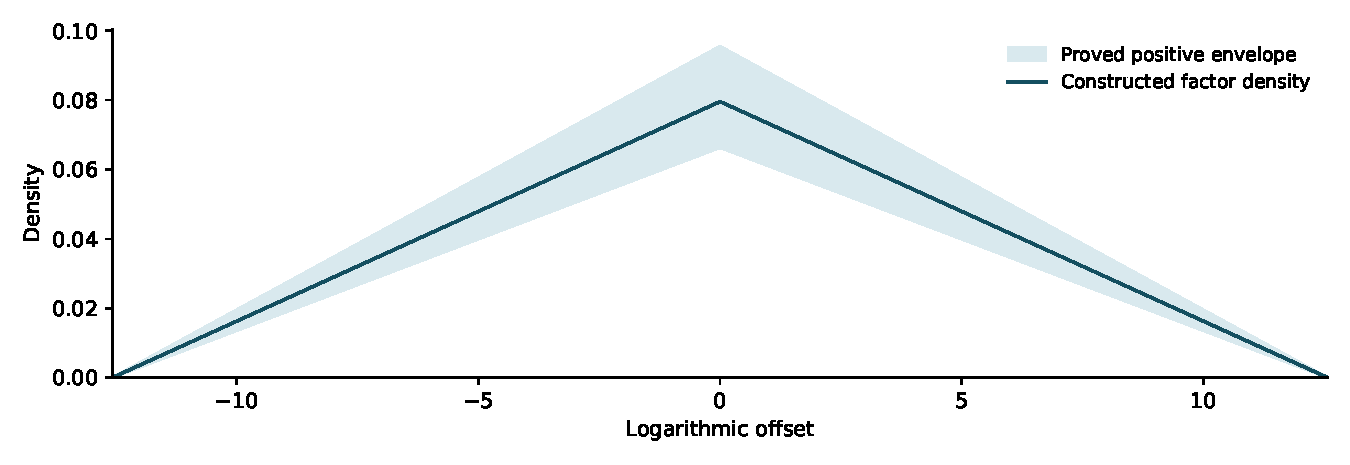
\includegraphics[width=\textwidth]{figures/positive_factor.pdf}
\caption{One interpolating density for the positive ordinates below
$100$ and their negatives. The shaded region is the proved envelope
between $5/6$ and $6/5$ times the triangular density. The display uses
numerical ordinates and coefficients; positivity of the exact
construction is proved independently.}
\end{figure}

\begin{figure}[htbp]
\centering
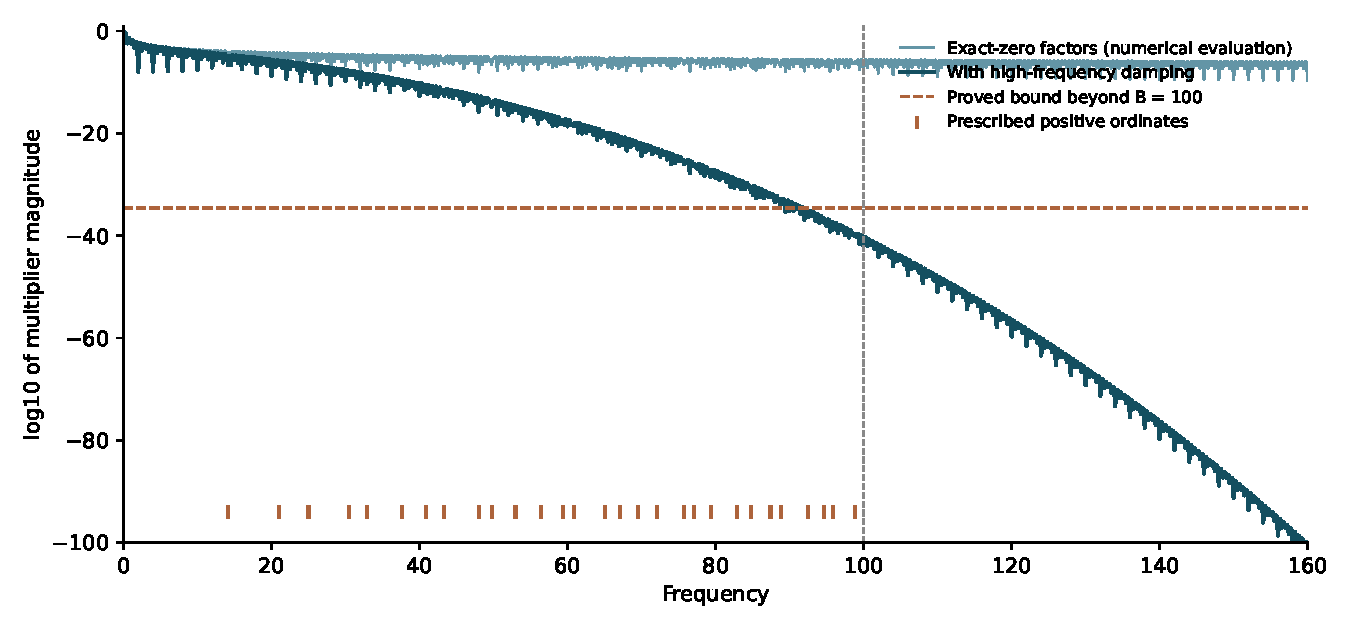
\includegraphics[width=\textwidth]{figures/filter_response.pdf}
\caption{Numerical frequency response for $B=100$. Tick marks along
the bottom indicate prescribed positive ordinates, where the exact
construction has zeros; the sampled curve need not hit those points.
The uniform-convolution factors supply the proved global damping bound
beyond the cutoff. Values below $10^{-100}$ are clipped for display.}
\end{figure}

\subsection{Formalization boundary}

The input RH and Dirichlet GRH statements belong to a separately checked
Lean development. The new positive-filter, support-optimality, and
prime-average proofs in this report have not been formalized in Lean.
The archive contains a detailed formalization roadmap, not a stub proof
with hidden axioms or \texttt{sorry} declarations. Its shortest independent
formal component would be the finite matrix lemma and exact positivity
margin; the deeper analytic dependencies are the local zero count,
Jensen's formula, and the contour form of the explicit formula.

% Input fragment. Requires hyperref (for \url), amsmath and amssymb.
% Companion bibliography entries are in references_extra.tex.

\section{Sources, prior methods, and the boundary of the contribution}
\label{sec:sources-literature}

\subsection{Positive interpolation is an established subject}

The construction in Section~\ref{sec:annihilation} does not originate
the general problem of Fourier interpolation by positive compactly
supported measures. Florek's 1987 paper has precisely that subject
in its title~\cite{Florek}. The publisher's bibliographic record was
available, but its full-text download returned an access error in
this investigation. Consequently, no specific quantitative theorem
is attributed to that paper and no claimed distinction rests on
guessing its contents.

As independently inspected context, Graham and Hare~\cite{GrahamHare}
study interpolation by nonnegative measures for Sidon,
$\varepsilon$-Kronecker and $I_0$ sets. Their introduction explicitly
identifies Florek's result as a Sidon-set predecessor. Such results
establish clear historical precedent for positive interpolation.
They do not, in the passages inspected, state the present support
bound for an arbitrary finite multiset in terms of its local
occupancy, with prescribed zero orders and a simultaneous uniform
tail estimate.

Kahane's treatment of nonharmonic Fourier series supplies a close
classical mechanism~\cite{Kahane}. Proposition~VI.2.1, on printed
page~131, gives a sufficient diagonal-dominance condition on the
Fourier Gram matrix of a compact positive measure for equivalence
between the coefficient $\ell^2$ norm and the associated integral
norm. Proposition~VI.2.2 gives the interpolation interpretation.
We use this as context for the matrix argument, without claiming
that those propositions themselves impose positivity on a new
interpolating density. In the present elementary proof the explicit
$\ell^1$ estimate on the correction coefficients is what preserves
positivity pointwise. Diagonal dominance, the Neumann series, and
convolution are all classical tools.

\subsection{Translate averaging and support bounds}

Kozma and Oravecz~\cite{KozmaOravecz}, Theorem~1, prove that a real
trigonometric polynomial with finite symmetric integer spectrum
$S\subset\mathbb Z^d\setminus\{0\}$ has a zero in every ball of
diameter $\sum_{\lambda\in S}(4\|\lambda\|_2)^{-1}$.
Their proof successively adds suitable translates to remove
frequencies while retaining positivity. The same elementary
frequency-removal operation is the dual counterpart of convolving
positive two-point measures. Although their stated theorem uses
integer frequencies, that removal step makes sense for real
frequencies as well. This is relevant precedent for a cost obtained
by summing reciprocal frequencies; it is not presented here as a
published local-occupancy bound for Dirichlet ordinates.

The comparison with the supplied arithmetic packet is narrower and
can be checked directly. Its explicit construction uses one
interval-convolution factor for each selected ordinate, with support
cost on the scale of $\sum_{0<\gamma\le B}\gamma^{-1}$, hence
$O((\log B)^2)$ for a fixed Dirichlet family. The construction proved
here groups occurrences into separated classes before convolution.
The local zero count bounds the number of classes by $O(\log B)$.
It thereby obtains support $O(\log B)$ while retaining exact
cancellation and adding the explicit tail attenuation. This is the
specific quantitative improvement over the inspected packet.

\subsection{The lower bound uses proved pair correlation only}

For multiplicity-preserving cancellation, Jensen's formula and the
Riemann--von Mangoldt count give the lower bound directly; simplicity
is irrelevant. For ordinary cancellation at distinct zeta ordinates,
Montgomery's proved squared-sinc pair-sum formula~\cite{Montgomery}
gives
\[
 \sum_{\gamma\ \mathrm{distinct},\ 0<\gamma\le T}m_\gamma^2
 \le (4/3+o(1))N(T).
\]
The parameter stays within the proved Fourier-support range and is
then allowed to approach its endpoint. No pair-correlation
conjecture is assumed. The integer inequality
$1\ge(3m-m^2)/2$ for $m\ge1$ yields the distinct-zero proportion
$5/6-o(1)$, also explicitly discussed by
Conrey--Ghosh--Gonek~\cite[pp.~497--498]{CGG}. This leads to the
convenient lower support constant $5/12$ for ordinary cancellation.
It is not asserted to be the strongest constant in the literature.

\subsection{Novelty and verification limits}

The claim supported by this packet is an explicitly proved
quantitative arithmetic improvement relative to the supplied
documents: logarithmic support, prescribed aggregate zero orders,
uniform high-frequency attenuation, and the resulting common
positive average of the smoothed residue-class errors. The
matching logarithmic obstruction explains the scale of the result.
The argument does not require independence of zero ordinates or
distinctness across different characters.

The literature search identified substantial related work and an
especially relevant older positive-interpolation paper whose full
text could not be inspected. Accordingly, global priority is
unverified. The packet claims neither a new general theory of
positive Fourier interpolation nor the solution of another named
conjecture. Numerical examples illustrate the finite construction;
the proofs, rather than numerical residuals, establish exact
cancellation.


\begin{thebibliography}{99}
\raggedright
\bibitem{grh}
L. Sernau and collaborators, \emph{GRH for Dirichlet $L$-functions, in
Lean 4}, commit \path{72fead102f663d5c7a407964a13dc0cf9d977207},
25 November 2026. \url{https://github.com/lsernau/grh-lean}.

\bibitem{leanstatement}
Lean FRO and Mathlib Initiative, \emph{Lean verification of the
Riemann Hypothesis}, joint statement, 21 November 2026.
\url{https://leanprover-community.github.io/blog/posts/riemann-hypothesis/}.

\bibitem{sutherland}
A. Sutherland, \emph{Verification files for the shorter Lean proof of
RH and of GRH for Dirichlet $L$-functions}, update of 26 November 2026,
20:46 UTC. \url{https://math.mit.edu/~drew/shortgrh/}.
The audit records the linked axiom and paranoid Comparator logs for
both exact editions; these records were inspected, not rerun locally.

\bibitem{catalogue}
V. Reshetnikov, \emph{ProveIt: Generalized Riemann Hypothesis research
catalogue}, commit \path{dedc2966ea6f59cc0a8fd0327d68cda31bce6df1},
inspected 26 November 2026, Pacific time.
\url{https://github.com/VladimirReshetnikov/ProveIt/tree/main/Analysis/GeneralizedRiemannHypothesis}.

\bibitem{priorbalance}
ProveIt research packet, \emph{Simultaneous balancing of prime errors
in bounded logarithmic windows}, 26 November 2026, at the commit of
\cite{catalogue}. Section 5 gives the earlier compact positive kernel.
\url{https://github.com/VladimirReshetnikov/ProveIt/blob/dedc2966ea6f59cc0a8fd0327d68cda31bce6df1/Analysis/GeneralizedRiemannHypothesis/Research/grh_prime_error_balancing/report.tex}.

\bibitem{wiki}
Wikipedia contributors, \emph{Riemann hypothesis}, accessed
26 November 2026. \url{https://en.wikipedia.org/wiki/Riemann_hypothesis}.
Requested overview; primary sources above support the proof-status claims.

\bibitem{Davenport}
H. Davenport, \emph{Multiplicative Number Theory}, 3rd edition,
revised by H. L. Montgomery, Graduate Texts in Mathematics 74,
Springer, 2000. Classical Dirichlet explicit formulas and zero counts.
\url{https://doi.org/10.1007/978-1-4757-5927-3}.

\bibitem{Florek}
J.~Florek,
\emph{Interpolation by the Fourier--Stieltjes transform of a positive compactly supported measure},
Colloquium Mathematicum \textbf{54} (1987), 113--120.
\href{https://doi.org/10.4064/cm-54-1-113-120}{doi:10.4064/cm-54-1-113-120}.
Publisher metadata inspected; full text was not available to this audit.

\bibitem{Kahane}
J.-P.~Kahane,
\emph{Pseudo-p\'eriodicit\'e et s\'eries de Fourier lacunaires},
Annales scientifiques de l'\'Ecole Normale Sup\'erieure, S\'erie~3,
\textbf{79} (1962), no.~2, 93--150.
\href{https://doi.org/10.24033/asens.1108}{doi:10.24033/asens.1108}.
\url{https://www.numdam.org/item/ASENS_1962_3_79_2_93_0.pdf}.

\bibitem{KozmaOravecz}
G.~Kozma and F.~Oravecz,
\emph{On the gaps between zeros of trigonometric polynomials},
Real Analysis Exchange \textbf{28} (2002/2003), no.~2, 447--454.
Author preprint: \url{https://arxiv.org/abs/math/0601021}.

\bibitem{Montgomery}
H.~L.~Montgomery,
\emph{The pair correlation of zeros of the zeta function},
in \emph{Analytic Number Theory}, Proceedings of Symposia in Pure
Mathematics \textbf{24}, American Mathematical Society, 1973,
181--193.
\url{https://public.websites.umich.edu/hlm/paircor1.pdf}.

\bibitem{CGG}
J.~B.~Conrey, A.~Ghosh and S.~M.~Gonek,
\emph{Simple zeros of the Riemann zeta-function},
Proceedings of the London Mathematical Society (3)
\textbf{76} (1998), 497--522.
\url{https://www.sas.rochester.edu/mth/people/faculty/gonek-steve/assets/pdf/simplezeros.pdf}.

\bibitem{GrahamHare}
C.~C.~Graham and K.~E.~Hare,
\emph{$\varepsilon$-Kronecker and $I_0$ sets in abelian groups, IV:
interpolation by non-negative measures},
Studia Mathematica \textbf{177} (2006), no.~1, 9--24.
\href{https://doi.org/10.4064/sm177-1-2}{doi:10.4064/sm177-1-2}.
The complete published paper was inspected through a PDF mirror.

\end{thebibliography}
\end{document}
